\documentclass[]{beamer}
\usepackage{graphicx}
\usepackage{algorithm}
\usepackage{algpseudocode}
\usepackage{amsmath, amsfonts, amssymb}

\newcommand{\abs}[1]{\left\lvert#1\right\rvert}

\newenvironment{fr}
               {\begin{frame}{\secname}}
               {\end{frame}}
\newenvironment{ffr}
               {\begin{frame}{\subsecname}}
               {\end{frame}}

\title{Thiết kế và phân tích giải thuật}
\author{Nguyễn Đức Hùng, Đỗ Ngọc Dũng, Nguyễn Quang Minh}
\begin{document}
\begin{frame}
\maketitle
\end{frame}
\begin{frame}{Outline}
\tableofcontents
\end{frame}

\section{Thuật toán}
\begin{fr}
  \begin{block}{Thuật toán}
    Thuật toán là tập hợp hữu hãn các chỉ dẫn nhằm giải quyết một vấn đề nào đó hoặc thực việc một công việc tính toán nào đó.
  \end{block}
  Thuật toán đại diện cho cách giải quyết một vấn đề, do đó độc lập với ngôn ngữ lập trình.
\end{fr}

\subsection{Các bước thiết kế thuật toán}
\begin{ffr}
  \begin{enumerate}
  \item Problem definition -- Định ra vấn đề
  \item Development of a model -- Mô hình hóa
  \item Specification of the algorithm -- Xác định đặc trưng
  \item Designing an algorithm -- Thiết kế thuật toán
  \item Checking the correctness of the algorithm -- Kiểm tra tính đúng đắn thuật toán
  \item Analysis of algorithm -- Phân tích thuật toán
  \item Implementation of algorithm -- Triển khai cài đặt thuật toán
  \item Program testing -- Kiểm thử
  \item Documentation preparation -- Tài liệu về thuật toán
  \end{enumerate}
\end{fr}

\subsection{Hương tiếp cận top -- down}
\begin{ffr}
    \begin{figure}
      \hfill
      \begin{minipage}{0.49\textwidth}
        \centering
        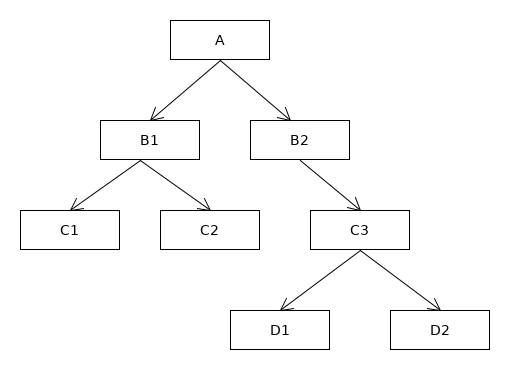
\includegraphics[width=\textwidth]{module-con.png}
      \end{minipage}
      \hfill 
      \begin{minipage}{0.49\textwidth}
        \centering
        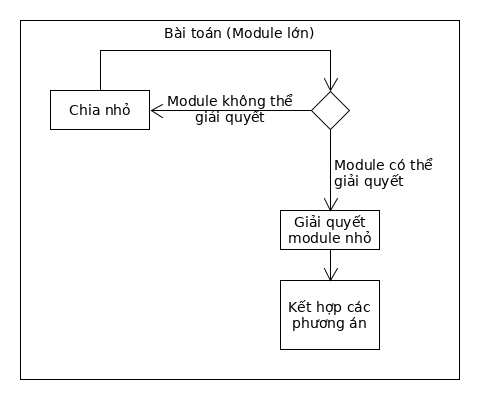
\includegraphics[width=\textwidth]{chia-nho.png}
      \end{minipage}
      \caption{\label{fig:chia-nho} Chia nhỏ bài toán thành các module cơ bản}
      \hfill
    \end{figure}
\end{ffr}

\subsection{Phương pháp tinh chỉnh từng bước}
\begin{ffr}
  \begin{block}
    {Tinh chỉnh từng bước} 
    Là phương pháp thiết kế giải thuật gắn liền với quá trình lập trình, phản ánh tinh thần của quá trình module hóa và thiết kế của top-down
  \end{block}
\end{ffr}
\begin{ffr}
\begin{enumerate}
  \item Thuật toán được thể hiện bằng lời lẽ tự nhiên của người thiết kế
  \item Tinh chỉnh lời ý chi tiết và gần với ngôn ngữ lập trình hơn (mã giả)
  \item Ngôn ngữ lập trình
\end{enumerate}
\end{ffr}

\begin{fr}
  Một số tính chất:
  \begin{itemize}
  \item Chính xác: đảm bảo kết quả trả về là đúng
  \item Rõ ràng: các bước thực hiện minh bạch
  \item Tính dừng: các bước thực hiện thuật toán là hữu hạn và thuật toán có điểm dừng
  \item Phổ dụng: có thể dễ dàng sửa đổi để thích ứng với các bài toán trong cùng một lớp và làm việc trên các dữ liệu đầu vào khác nhau
  \item Tính khả thi: bộ nhớ yêu cầu đủ nhỏ, thuật toán có thể cài đặt được, thực hiện trong thời gian cho phép\ldots
  \end{itemize}
  Cách biểu diễn thuật toán 
  \begin{itemize}
  \item Lời nói
  \item Flowchart
  \item Mã giả (pseudo code)
  \end{itemize}
\end{fr}

\subsection{Phân loại thuật toán}
\begin{ffr}
  \begin{itemize}
  \item Brute-force
  \item Divide and conquer
  \item Search and enumeration
  \item Randomized algorithm
  \item Reduction of complexity
  \item Back tracking
  \item Heuristic
  \end{itemize}
\end{ffr}

\begin{frame}{Ví dụ}
  \begin{figure}[ht]
    \begin{minipage}{0.3\textwidth}
      \centering
      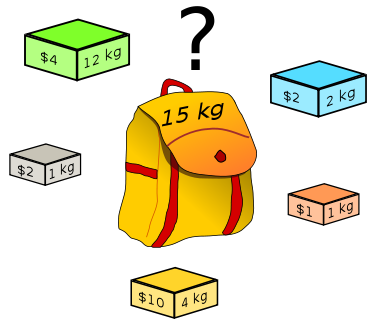
\includegraphics[height=0.3\pageheight]{knapsack.png}
      \caption{Bài toán cái túi}
    \end{minipage}
    \hfill
    \begin{minipage}{0.65\textwidth}
      \begin{algorithm}[H]
        \caption{Giải thuật tham lam}
        \begin{algorithmic}[1]
          \Procedure{Greedy}{$value, weight, W$}
          \State {Tính $cost = \frac{value}{weight}$ của mỗi vật}
          \While {$TotalWeight < W$}
          \State {Lấy vật có $cost$ cao nhất}
          \EndWhile
          \EndProcedure
        \end{algorithmic}
      \end{algorithm}
    \end{minipage}
  \end{figure}
\end{frame}

\section{Phân tích thuật toán}
\begin{fr}
  \begin{itemize}
  \item Phân tích tính đúng đắn
  \item Phân tích thời gian thực hiện
  \item Phân tích không gian (bộ nhớ cần dùng)
  \end{itemize}
\end{fr}

\subsection{Phân tích thuật toán về thời gian thực hiện}
\begin{ffr}
  \begin{block}{Thời gian thực hiện thuật toán}
  Thời gian thực hiện được tính bằng số {\it phép tính cơ bản} được sử dụng để xử lý đầu vào với một {\it kích thước} nào đó.
  \end{block}\medskip{}
  Ví dụ:
  \begin{description}
  \item[phép cộng 2 số nguyên] là một phép toán cơ bản.
  \item[phép cộng 2 vector] {\it không} phải là một phép toán cơ bản.
  \end{description}
  Kí hiệu:
  \begin{itemize}
  \item Kích thước dữ liệu đầu vào $n$
  \item Thời gian thực hiện giải thuật $T(n)$
  \end{itemize}
\end{ffr}

\begin{ffr}
  \begin{figure}[ht]
    \centering
    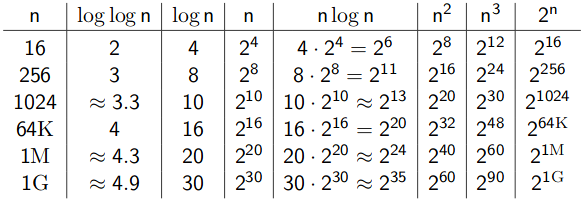
\includegraphics[width=\textwidth]{complex.png}
    \caption{\label{fig:label} Số phép tính cơ bản với độ lớn của dữ liệu đầu vào tương ứng}
  \end{figure}
\end{ffr}

\begin{ffr}
  Phân tích tiệm cận:
  \begin{itemize}
  \item $f(n) \in O(g(n)) \iff \exists C_1,n_o,\ \forall n > n_o: \abs{f(n)} \le C_1 \abs{g(n)}$
  \item $f(n) \in \Omega(g(n)) \iff \exists C_2,\ n_o, \forall n > n_o: \abs{f(n)} \ge C_2 \abs{g(n)}$
  \item $f(n) = \Theta(g(n)) \iff f(n) \in O(g(n)) \land f(n) \in \Omega(g(n))$ 
  \end{itemize}
  Các quy tắc:
  \begin{itemize}
  \item Quy tắc tổng
  \item Quy tắc nhân
  \end{itemize}
\end{ffr}

\begin{ffr}
  Thời gian thực hiện giải thuật trung bình
  \begin{itemize}
  \item Kịch bản tốt nhất
  \item Kịch bản xấu nhất
  \item Trường hợp trung bình
  \end{itemize}
\end{ffr}

\subsection{Phân tích thuật toán về mặt không gian}
\begin{ffr}
  \begin{block}{Space -- time tradeoff}
    Không gian bộ nhớ chiếm dụng cũng rất quan trọng. Khi tối ưu không gian chiếm dụng, ta có thể gặp phải vấn đề space/time tradeoff -- đánh đổi giữa không gian chiếm dụng và thời gian tính toán. 
  \end{block}
  \textbf{Ví dụ:} Tính giai thừa của một số.\vspace{-1em}
  \begin{minipage}[t]{0.4\pagewidth}
    \begin{algorithm}[H]
      \caption{Tính chay}
      \begin{algorithmic}[1]
        \Procedure{Giai thừa}{m}
        \State $n = 1$
        \For{$i=2$ \textbf{to} $m$}
        \State {$n = n \times i$}
        \EndFor
        \State {\bf Return $n$}
        \EndProcedure
      \end{algorithmic}
    \end{algorithm}
  \end{minipage}
  \begin{minipage}[t]{0.4\pagewidth}
    \begin{algorithm}[H]
      \caption{Lookup}
      \begin{algorithmic}[1]
        \State $facts = [1, 2, 6, 24,\ldots] $
        \Procedure{Giai thừa}{n}
        \State {\bf Return $facts[n]$}
        \EndProcedure
      \end{algorithmic}
    \end{algorithm}
  \end{minipage}
\end{ffr}

\subsection{Phân tích với nhiều tham só}
\begin{ffr}
  Đôi lúc bài giải thuật của chúng ta có độ phức tạp cần được đánh giá bằng nhiều tham số
  \begin{block}{Bài toán ví dụ}
    Cho một bức ảnh có $n$ pixel với $m$ màu khác nhau, đếm số lần xuất hiện của mỗi màu trong ảnh.
  \end{block}
  \begin{algorithm}[H]
    \caption{Đếm màu}
    \begin{algorithmic}[1]
        \For{$i = 1:m$}
        \State {count[i] = 0}
        \EndFor
        \For{$i = 1:n$}
        \State {count[value(i)] ++}
        \EndFor
    \end{algorithmic}
  \end{algorithm}
\end{ffr}
\end{document}
